% 04-structurPlan
\section{Projektstrukturplan}
\begin{frame}
	\frametitle{Projektstrukturplan}
	
	\tikzset{
		basic/.style  = {draw, scale = 0.65, rectangle},
		root/.style   = {basic, rounded corners=2pt, top color=white, bottom color=blue!20},
		level 2/.style = {basic, rounded corners=4pt, thin,align=center, top color=white, bottom color=green!20},
		level 3/.style = {basic, thin, align=left, top color=white, bottom color=red!20, text width=7.4em}
	}
	\bigskip
	\bigskip
	\bigskip

	\centering
		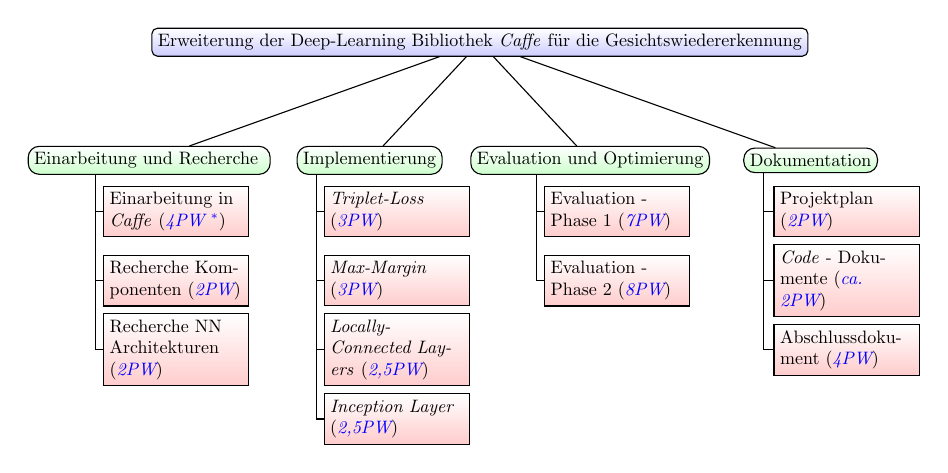
\begin{tikzpicture}[
		level 1/.style={sibling distance=28mm},
		edge from parent/.style={-,draw},
		>=latex]
		
		% root of the the initial tree, level 1
		\node[root] {Erweiterung der Deep-Learning Bibliothek \textit{Caffe} f\"ur die Gesichtswiedererkennung}
		% The first level, as children of the initial tree
		child {node[level 2] (c1) {Einarbeitung und Recherche }}
		child {node[level 2] (c2) {Implementierung}}
		child {node[level 2] (c3) {Evaluation und Optimierung}}
		child {node[level 2] (c4) {Dokumentation}};
		
		% The second level, relatively positioned nodes
		\begin{scope}[every node/.style={level 3}]
		\node [below of = c1, xshift = 15pt] (c11) {Einarbeitung in \textit{Caffe} (\textit{\textcolor{blue}{4PW $^*$}})};
		\node [below of = c11, yshift = -10pt] (c12) {Recherche Komponenten (\textit{\textcolor{blue}{2PW}})};
		\node [below of = c12, yshift = -10pt] (c13) {Recherche NN Architekturen (\textit{\textcolor{blue}{2PW}})};
		
		\node [below of = c2, xshift = 15pt] (c21) {\textit{Triplet-Loss} (\textit{\textcolor{blue}{3PW}})};
		\node [below of = c21, yshift = -10pt] (c22) {\textit{Max-Margin} (\textit{\textcolor{blue}{3PW}})};
		\node [below of = c22, yshift = -10pt] (c23) {\textit{Locally-Connected Layers} (\textit{\textcolor{blue}{2,5PW}}) };
		\node [below of = c23, yshift = -10pt] (c24) {\textit{Inception Layer} (\textit{\textcolor{blue}{2,5PW}})};
		
		\node [below of = c3, xshift = 15pt] (c31) {Evaluation - Phase 1 (\textit{\textcolor{blue}{7PW}})};
		\node [below of = c31, yshift = -10pt] (c32) {Evaluation - Phase 2 (\textit{\textcolor{blue}{8PW}})};
		
		\node [below of = c4, xshift = 20pt] (c41) {Projektplan (\textit{\textcolor{blue}{2PW}})};
		% The time for code-Document is already included in implementation, so here is ''ca.".
		\node [below of = c41, yshift = -10pt] (c42) {\textit{Code} - Dokumente (\textit{\textcolor{blue}{ca. 2PW}})};
		\node [below of = c42, yshift = -10pt] (c43) {Abschlussdoku-\\ment (\textit{\textcolor{blue}{4PW}})};
		
		\end{scope}
		
		% lines from each level 1 node to every one of its "children"
		\foreach \value in {1,2,3}
		\draw[-] (c1.195) |- (c1\value.west);
		
		\foreach \value in {1,...,4}
		\draw[-] (c2.195) |- (c2\value.west);
		
		\foreach \value in {1,...,2}
		\draw[-] (c3.195) |- (c3\value.west);
		
		\foreach \value in {1,...,3}
		\draw[-] (c4.195) |- (c4\value.west);
		
	
	
	\end{tikzpicture}
	
	\begin{flushleft}
	
		\bigskip
		\bigskip
		\bigskip
		\tiny \textcolor{black}{* \textit{PW} ist die Abkurzung von \textit{ \glqq Personenwochen\grqq }}
	\end{flushleft}
	
	
	
	
\end{frame}